\documentclass[english]{article}
\usepackage[round]{natbib}
\bibliographystyle{abbrvnat}
%\usepackage{thumbpdf}
\usepackage{hyperref}

\usepackage{Sweave}
\begin{document}
\Sconcordance{concordance:statTarget.tex:statTarget.Rnw:%
1 6 1 1 0 92 1 1 2 5 0 1 2 1 4 2 1}


\author{Hemi Luan}

\title{statTarget:\\Statistical Analysis of Metabolite Profile}
%\VignetteIndexEntry{Introduction to statTarget}

\maketitle

\tableofcontents

\section{statTarget installation guide}

statTarget package needs GTK2 libraries to run.
Below, it is described how to install GTK2 libraries on Mac OS and Windows. \\

\subsection{For Mac OS users}


\noindent 1 - Install \texttt{Xcode} developer tools (at least version 5.0.1) from Apple Store (it is free).\\

\noindent 2 - Install \texttt{XQuartz-2.7.5.dmg} from  \texttt{http://xquartz.macosforge.org/landing/} \\

\noindent 3 - Install \texttt{GTK}$\_$\texttt{2.24.17}$\_$\texttt{X11.pkg} from \texttt{http://r.research.att.com} .\\

\noindent 4 - install.packages(""statTarget") .\\

\noindent 5 - library(statTarget)


\subsection{For Windows users}

\noindent 1 - download \texttt{gtk+-bundle}$\_$\texttt{2.22.1-20101229}$\_$\texttt{win64.zip} from \newline
\texttt{http://ftp.gnome.org/pub/gnome/binaries/win64/gtk+/2.22/} . \\

\noindent 2 - This is a bundle containing the GTK+ stack and its dependencies for Windows. To use it, create some empty folder like \texttt{$C:\backslash opt \backslash gtk$} .\\

\noindent 3 - Unzip this bundle.\\

\noindent 4 - Now, you have to add the bin folder to your \texttt{PATH} variable. Make sure you have no other versions of \texttt{GTK+} in \texttt{PATH} variable. To do this, execute the following instructions:
Open \texttt{Control Panel}, click on \texttt{System and Security}, click on \texttt{System}, click on \texttt{Advanced System Settings}, click on \texttt{Environment Variables}. In the \texttt{Environment Variables} window you will notice two columns \texttt{User variables} for a user name and \texttt{System variables}. Change the \texttt{PATH} variable in the \texttt{System variables} to be \texttt{$C:\backslash opt \backslash gtk \backslash bin$} .\\

This is all you need to install the GTK2 libraries.\\

\noindent 5 - install.packages("statTarget") .\\

\noindent 6 - library(statTarget).



\section[Overview of statTarget]{Overview of statTarget}

%
\begin{figure}

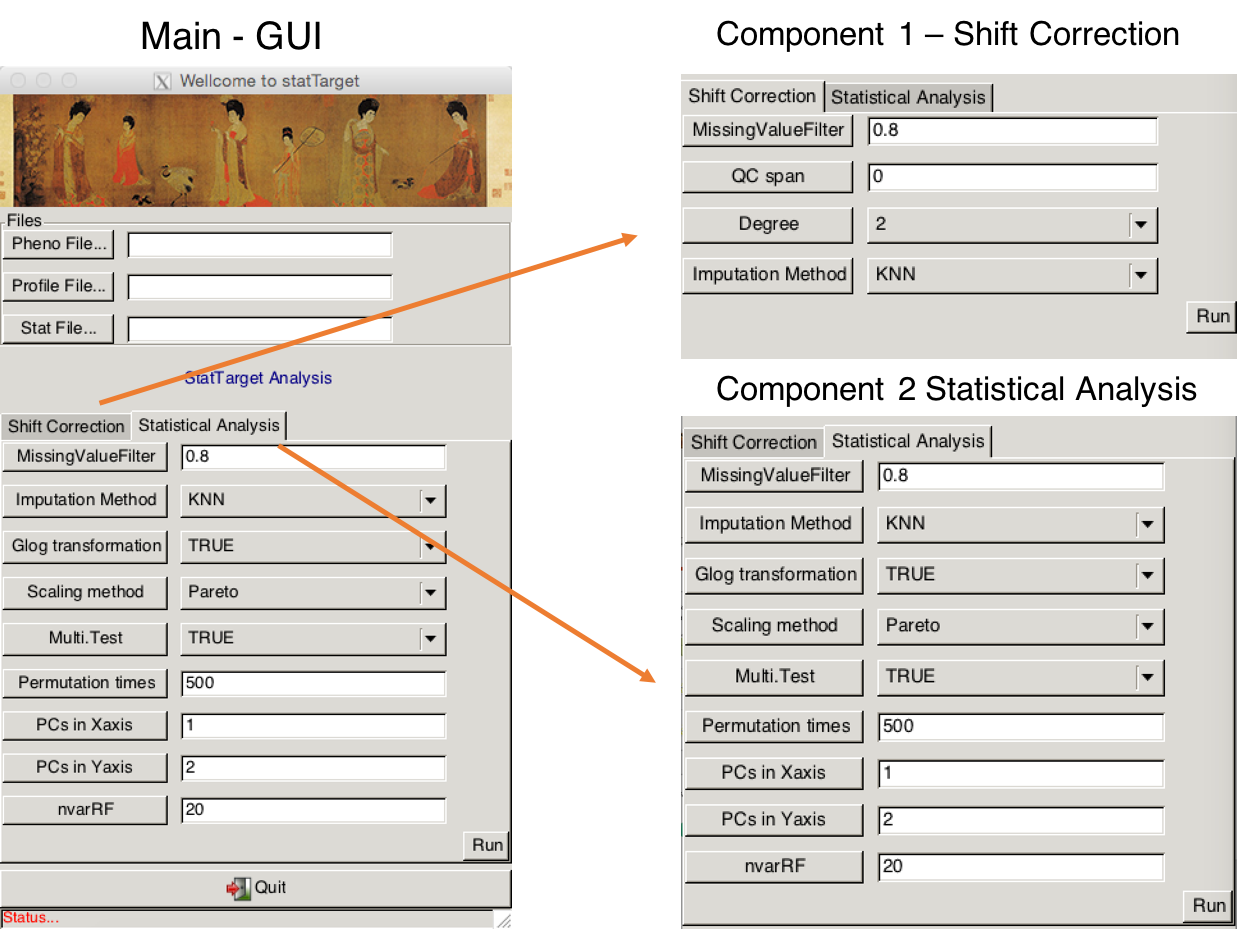
\includegraphics[scale=0.5]{main_gui}

\caption{\label{fig:main_gui}The main GUI of statTarget}

\end{figure}


A graphical user interface, easy to use tool provide quality control based signal correction, integration of metabolomic data from multiple batches, and the comprehensive statistic analysis for non-targeted and targeted approaches. The user controls statTarget through a Graphical User Interface (GUI), which 
is shown in Figure \ref{fig:main_gui}. 


\section[statTarget in detail]{statTarget in detail}


The main GUI of statTarget, shown in Figure \ref{fig:main_gui},
has two basic components. The first is shift correction. It includes quality control-based robust LOESS signal correction (QC-RLSC) that is a widely accepted method for quality control based signal correction and integration of metabolomic data from multiple analytical batches (Dunn WB., et al. 2011; Luan H., et al. 2015).\\ 

\subsection[statTarget Shift Correction]{statTarget Shift Correction}

statTarget - Shift Correction (Figure \ref{fig:main_gui}) provide QC-RLSC algorithm that fit the QC data, and each metabolites in the true sample will be normalized to the QC sample. Additonally, LOESS based generalised cross-validation (GCV) would be automatically applied to avoid overfitting of the observed data, when the QCspan was set at 0.\\ 

\subsection[statTarget Statistical Analysis]{statTarget Statistical Analysis}

statTarget - Statistical Analysis (Figure \ref{fig:main_gui}) provide features including Data preprocessing, Data descriptions, Multivariate statistics analysis and Univariate analysis.\\
Data preprocessing : 80-precent rule, log transformation, KNN imputation, Median imputation and Minimum values imputation.\\
Data descriptions :  Mean value, Median value, Sum, Quartile, Standard derivatives, etc.\\
Multivariate statistics analysis : PCA, PLSDA, OPLSDA, VIP, Random forest.
Univariate analysis : Student T-test, Shapiro-Wilk normality test and Mann-Whitney tests.\\
Biomarkers analysis for Clinical research : ROC, Odd ratio.




 
 
\section{Session Info}

\begin{itemize}\raggedright
  \item R version 3.3.0 (2016-05-03), \verb|x86_64-apple-darwin13.4.0|
  \item Locale: \verb|C/en_US.UTF-8/en_US.UTF-8/C/en_US.UTF-8/en_US.UTF-8|
  \item Base packages: base, datasets, grDevices, graphics, methods,
    stats, utils
  \item Loaded via a namespace (and not attached): tools~3.3.0
\end{itemize}


\end{document}
